\chapter{Projekt}


\section{Harmonogram}
Poniżej przedstawiony został harmonogram projektu wraz z diagramem Gantta.

  \begin{longtable}{| p{.40\textwidth} || p{.25\textwidth} | p{.25\textwidth} |}
\hline
\textbf{Nazwa zadania} & \textbf{Data rozpoczęcia} & \textbf{Data zakończenia} \\ \hline
Organizacja struktury projektu & 16-03-21 & 16-03-29 \\ \hline
Pierwsze spotkanie projektowe & 16-03-31 & 16-03-31 \\ \hline
Wystartowanie repozytorium Git & 16-04-01 & 16-04-04 \\ \hline
Ustalenia funkcjonalne i niefunkcjonalne & 16-04-01 & 16-04-05 \\ \hline
Utworzenie koncepcji architektury systemu & 16-04-01 & 16-04-20 \\ \hline
Utworzenie koncepcji wykorzystania narzędzia docker & 16-04-01 & 16-04-20 \\ \hline
Utworzenie dokumentu dobrych praktyk & 16-04-15 & 16-04-21 \\ \hline
Utworzenie tutoriala docker & 16-04-18 & 16-04-21 \\ \hline
Dodanie rozwiązania docker do repozytorium & 16-04-19 & 16-04-20 \\ \hline
Doprecyzowanie wymagań przedmiotu & 16-04-19 & 16-04-20 \\ \hline
Wybranie algorytmów & 16-04-19 & 16-04-20 \\ \hline
Ustalenie prezentacji na drugi krok milowy & 16-04-21 & 16-04-21 \\ \hline
Modułowy podział projektu & 16-04-21 & 16-04-22 \\ \hline
Szczegłowa koncepcja rozwiązania & 16-04-25 & 16-04-28 \\ \hline
Ustawienie środowiska programistycznego & 16-04-20 & 16-04-20 \\ \hline
Utworzenie pierwszych scenariuszy testowych (do prezentacji pierwszego kroku milowego) & 16-04-19 & 16-04-22 \\ \hline
Ustalenie wykorzystywanej bazy danych & 16-04-21 & 16-04-25 \\ \hline
Postawienie bazy danych & 16-04-26 & 16-04-27 \\ \hline
Część programistyczna & 16-04-25 & 16-06-03 \\ \hline
Zebranie dokumentacji na pierwszy krok & 16-04-22 & 16-04-22 \\ \hline
I krok milowy & 16-04-29 & 16-04-29 \\ \hline
Utworzenie wszystkich scenariuszy testowych & 16-04-25 & 16-05-03 \\ \hline
Odłożenie bruncha na II krok milowy & 16-04-29 & 16-04-29 \\ \hline
II krok milowy & 16-05-06 & 16-05-06 \\ \hline
Ustalenie prezentacji na trzeci krok milowy & 16-05-09 & 16-05-11 \\ \hline
Testy bezpieczeństwa & 16-05-30 & 16-06-03 \\ \hline
Testy fukcjonalne & 16-05-30 & 16-06-03 \\ \hline
Testy awaryjności & 16-05-30 & 16-06-03 \\ \hline
III krok milowy & 16-06-10 & 16-06-10 \\ \hline
Doprecyzowanie wymagań funkcjonalnych systemu & 16-05-05 & 16-05-06 \\ \hline
Doprecyzowanie wymagań niefunkcjonalnych systemu & 16-05-10 & 16-05-13 \\ \hline
Doprecyzowanie architektury systemu & 16-05-10 & 16-05-16 \\ \hline
Opracowanie pełnego planu testów & 16-05-09 & 16-05-20 \\ \hline
Opracowanie scenariusza końcowej prezentacji & 16-05-09 & 16-05-20 \\ \hline
Wyodrębnienie głównych elementów systemu & 16-05-15 & 16-05-15 \\ \hline
Określenie sposobu lokalnego developmentu aplikacji & 16-05-15 & 16-05-16 \\ \hline
Klient - użytkownik & 16-05-15 & 16-05-16 \\ \hline
Klient do wprowadzania danych & 16-05-20 & 16-05-31 \\ \hline
Węzeł zewnętrzny & 16-05-20 & 16-05-26 \\ \hline
Węzeł wewnętrzny & 16-05-23 & 16-05-26 \\ \hline
Algorytm elekcji & 16-05-23 & 16-05-31 \\ \hline
Protokół spójności & 16-05-27 & 16-05-31 \\ \hline
Protokół komunikacyjny & 16-05-15 & 16-05-20 \\ \hline
Baza danych & 16-05-15 & 16-05-20 \\ \hline
Przetwarzanie danych & 16-05-26 & 16-05-31 \\ \hline

\caption{Harmonogram projektu}
\label{tab:harmonogram}
\end{longtable} 


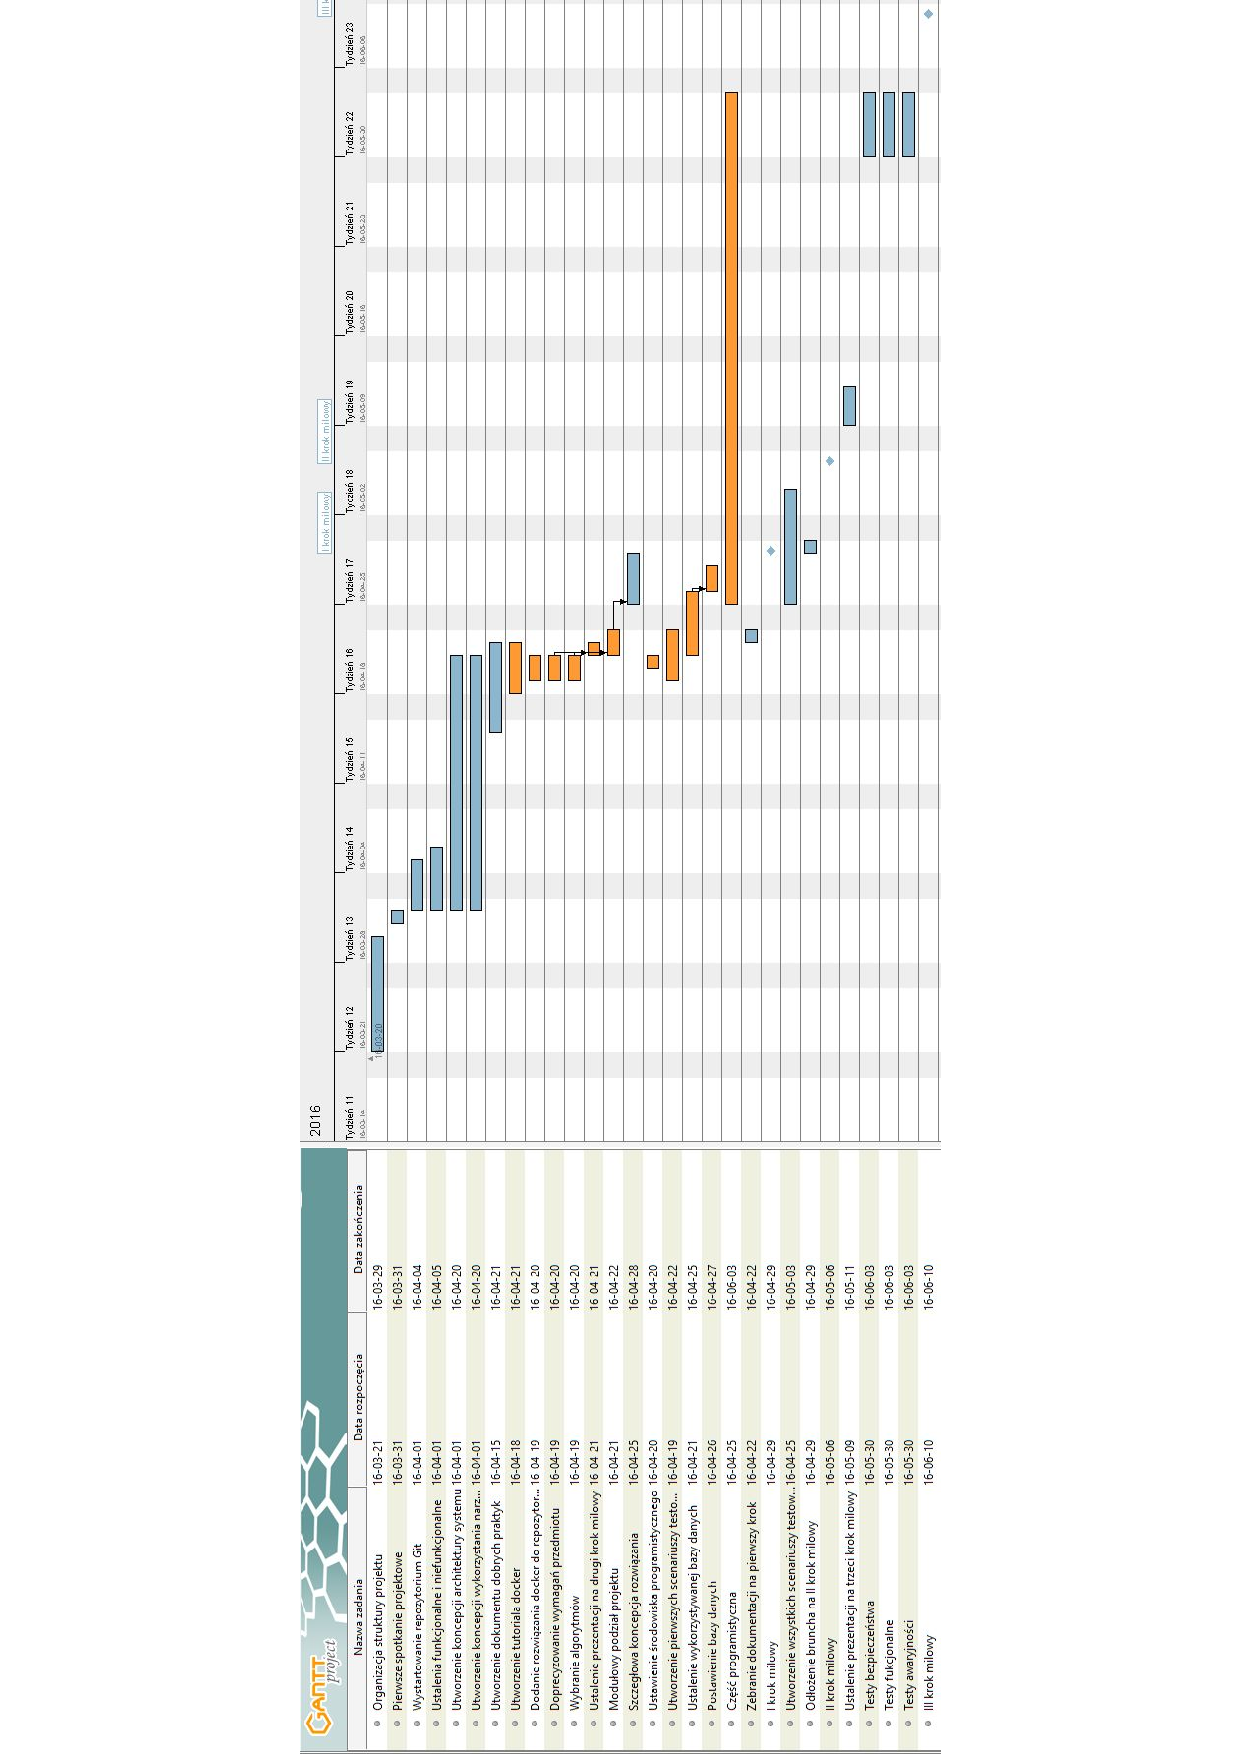
\includepdf[pages={1}]{pdf/gantt.pdf}
